\section{Implementation and results}\label{sec:results}
\subsection{Task 1: Model development}
\begin{figure}[ht]
    \begin{subfigure}{.5\textwidth}
        \centering
        % include first image
        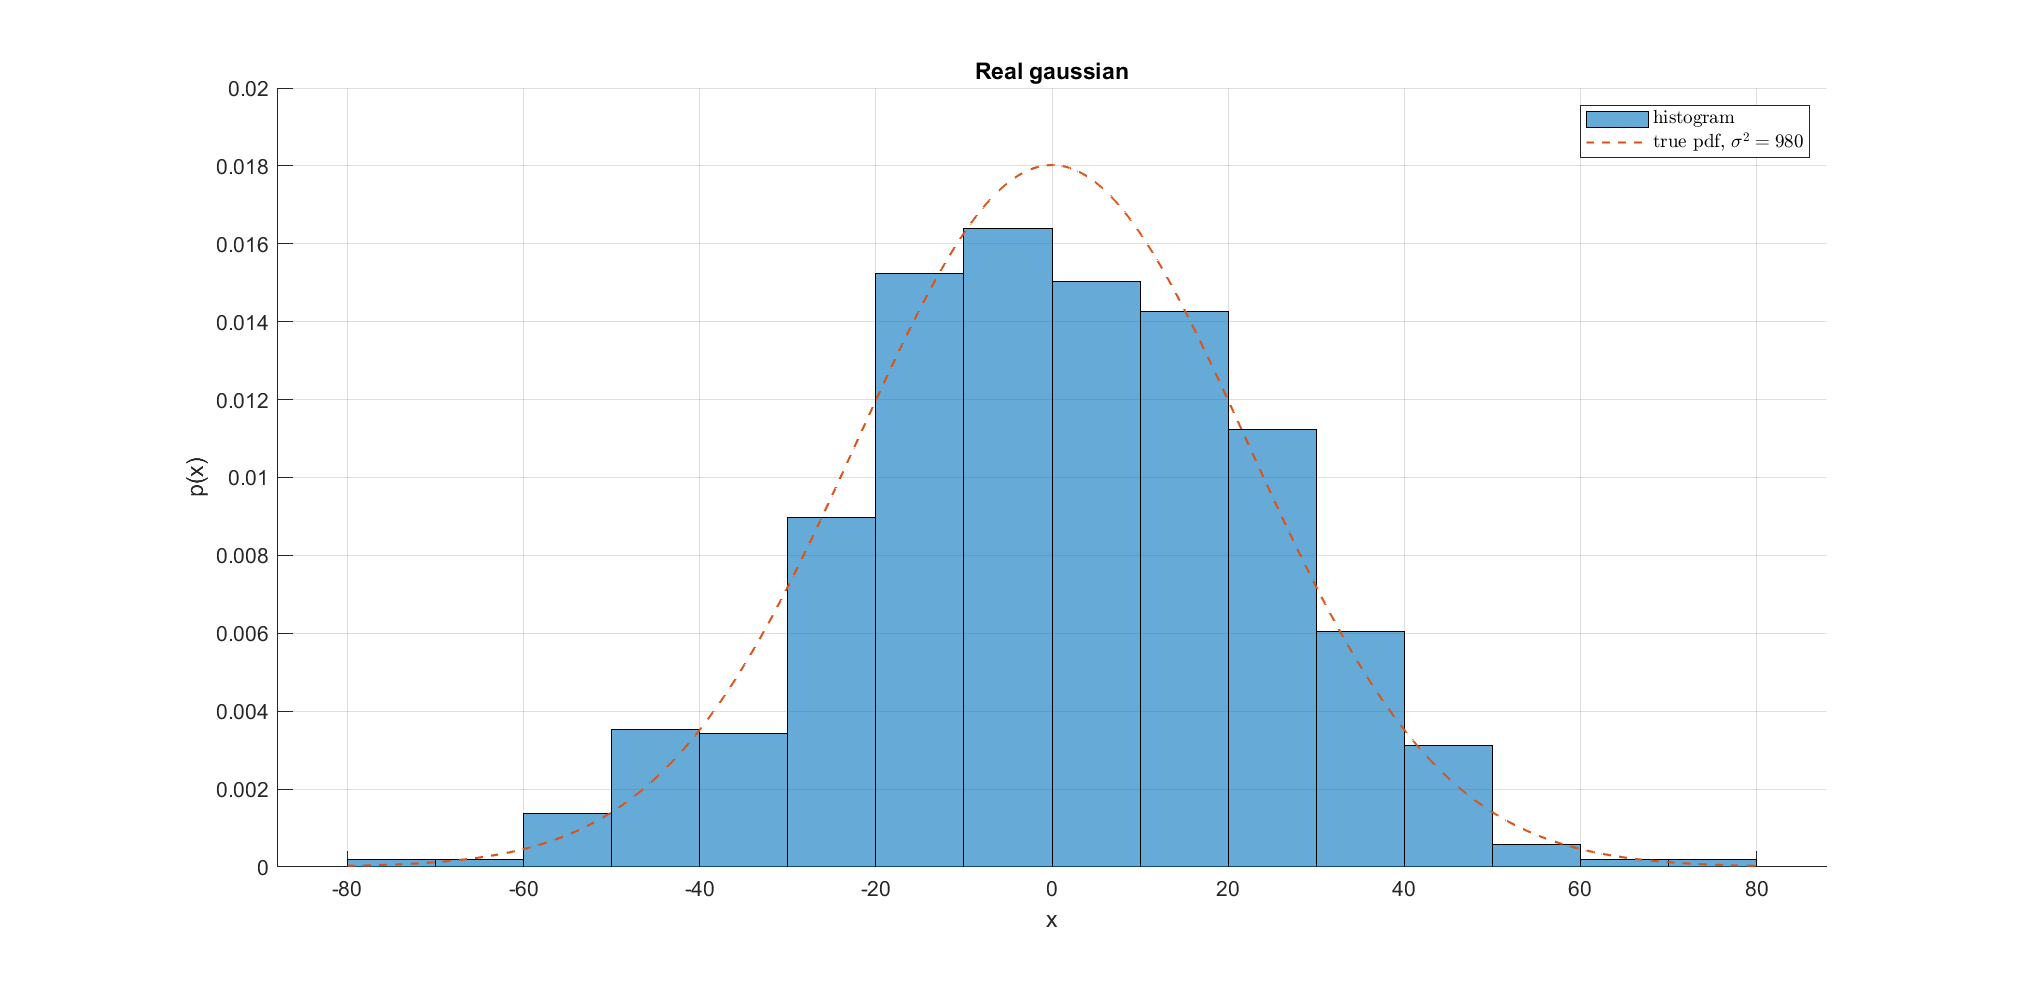
\includegraphics[width=.8\linewidth]{figures/re_gauss.eps}  
        \caption{The histogram of Re(S(k))$~$Gaussian}
        \label{fig:re_gauss}
    \end{subfigure}
    \begin{subfigure}{.5\textwidth}
        \centering
        % include second image
        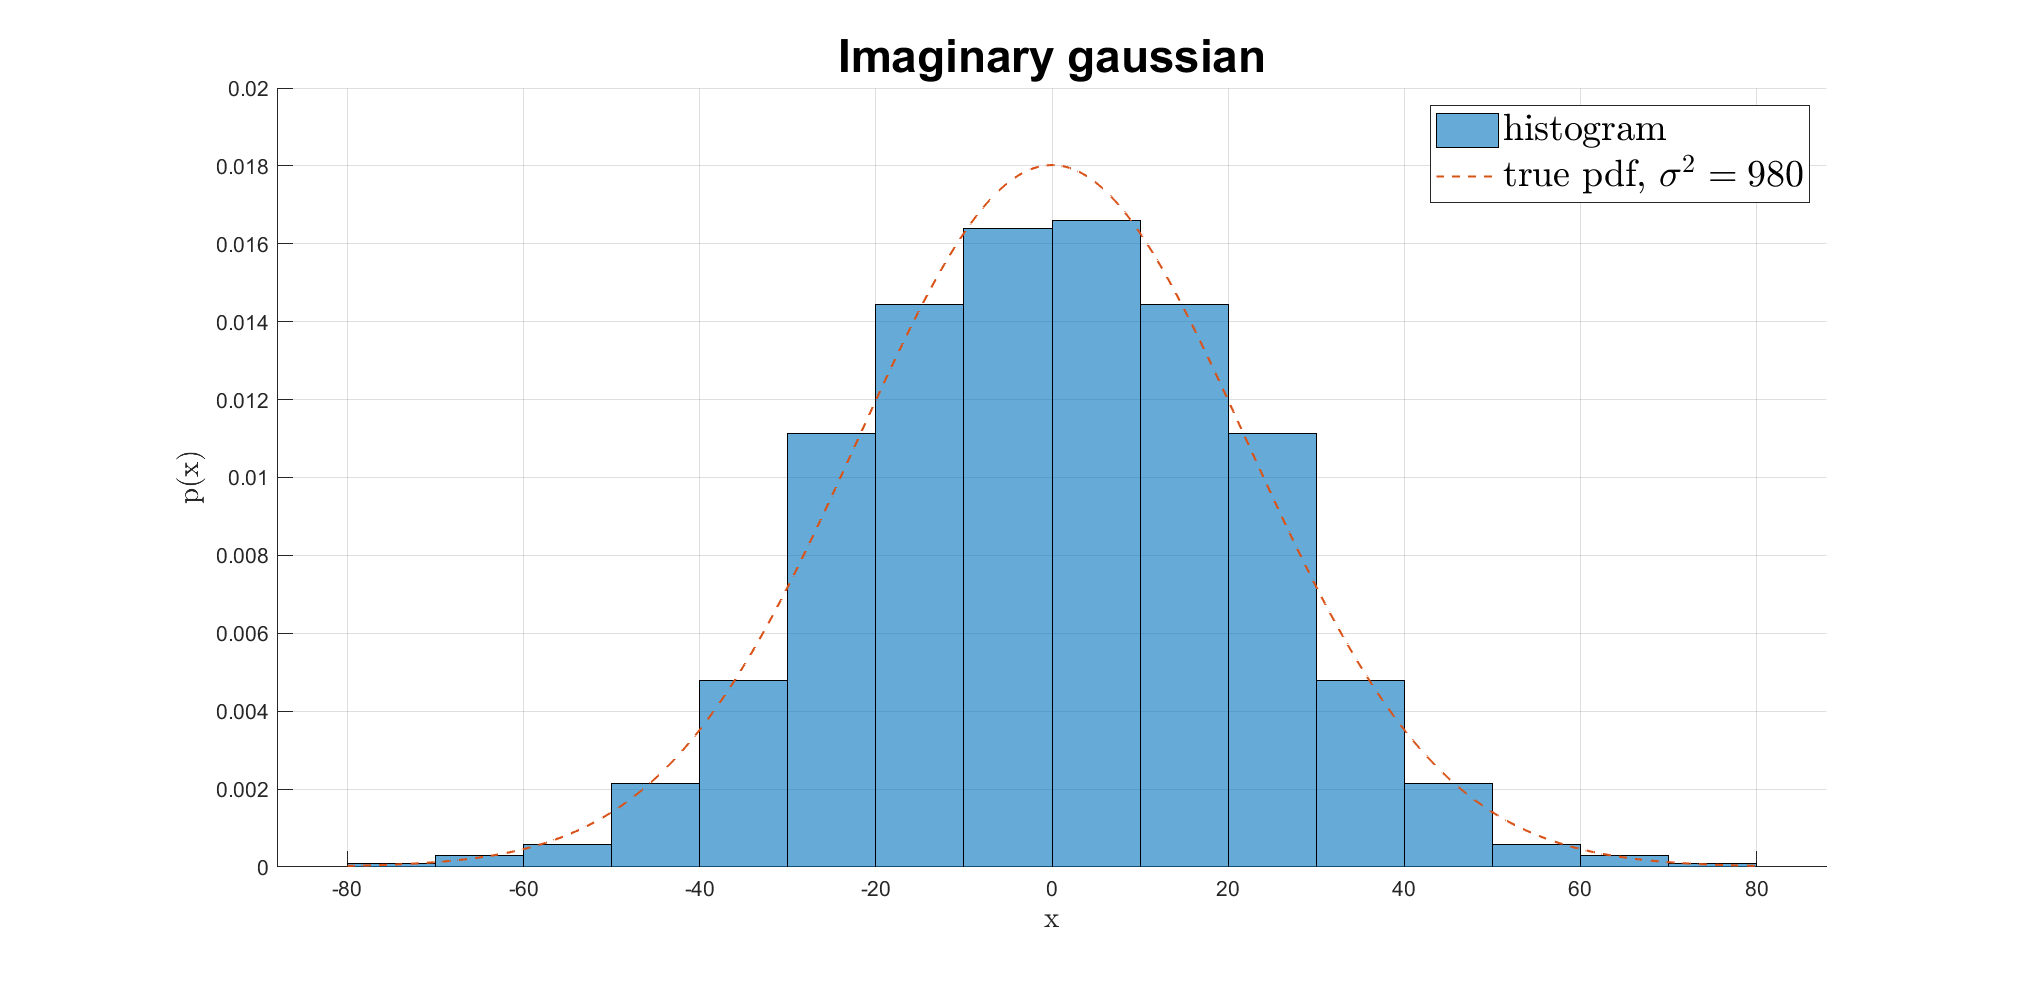
\includegraphics[width=.8\linewidth]{figures/im_gauss.eps}  
        \caption{The histogram of Im(S(k))$~$Gaussian}
        \label{fig:im_gauss}
    \end{subfigure}
    \begin{subfigure}{.5\textwidth}
        \centering
        % include third image
        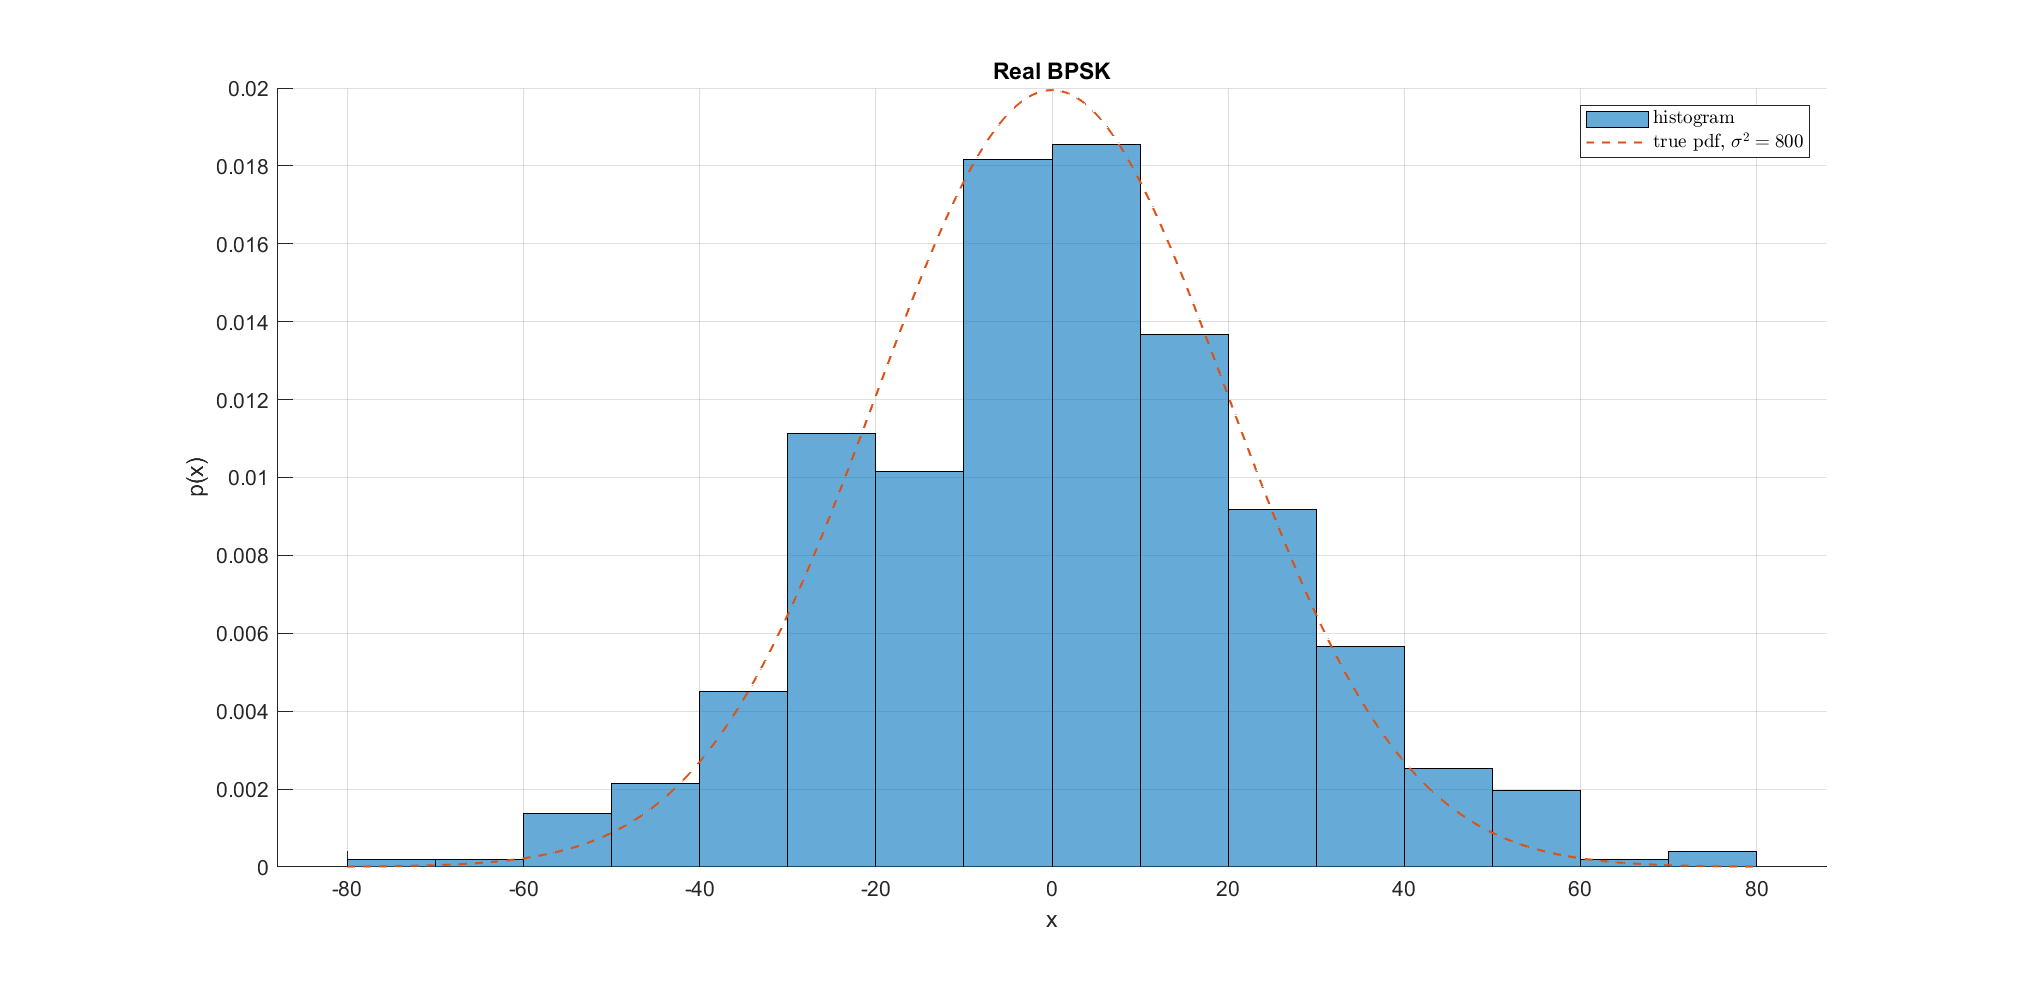
\includegraphics[width=.8\linewidth]{figures/re_bpsk.eps}
        \caption{The histogram of Re(S(k))$~$BPSK}
        \label{fig:re_bpsk}
    \end{subfigure}
    \begin{subfigure}{.5\textwidth}
        \centering
        % include fourth image
        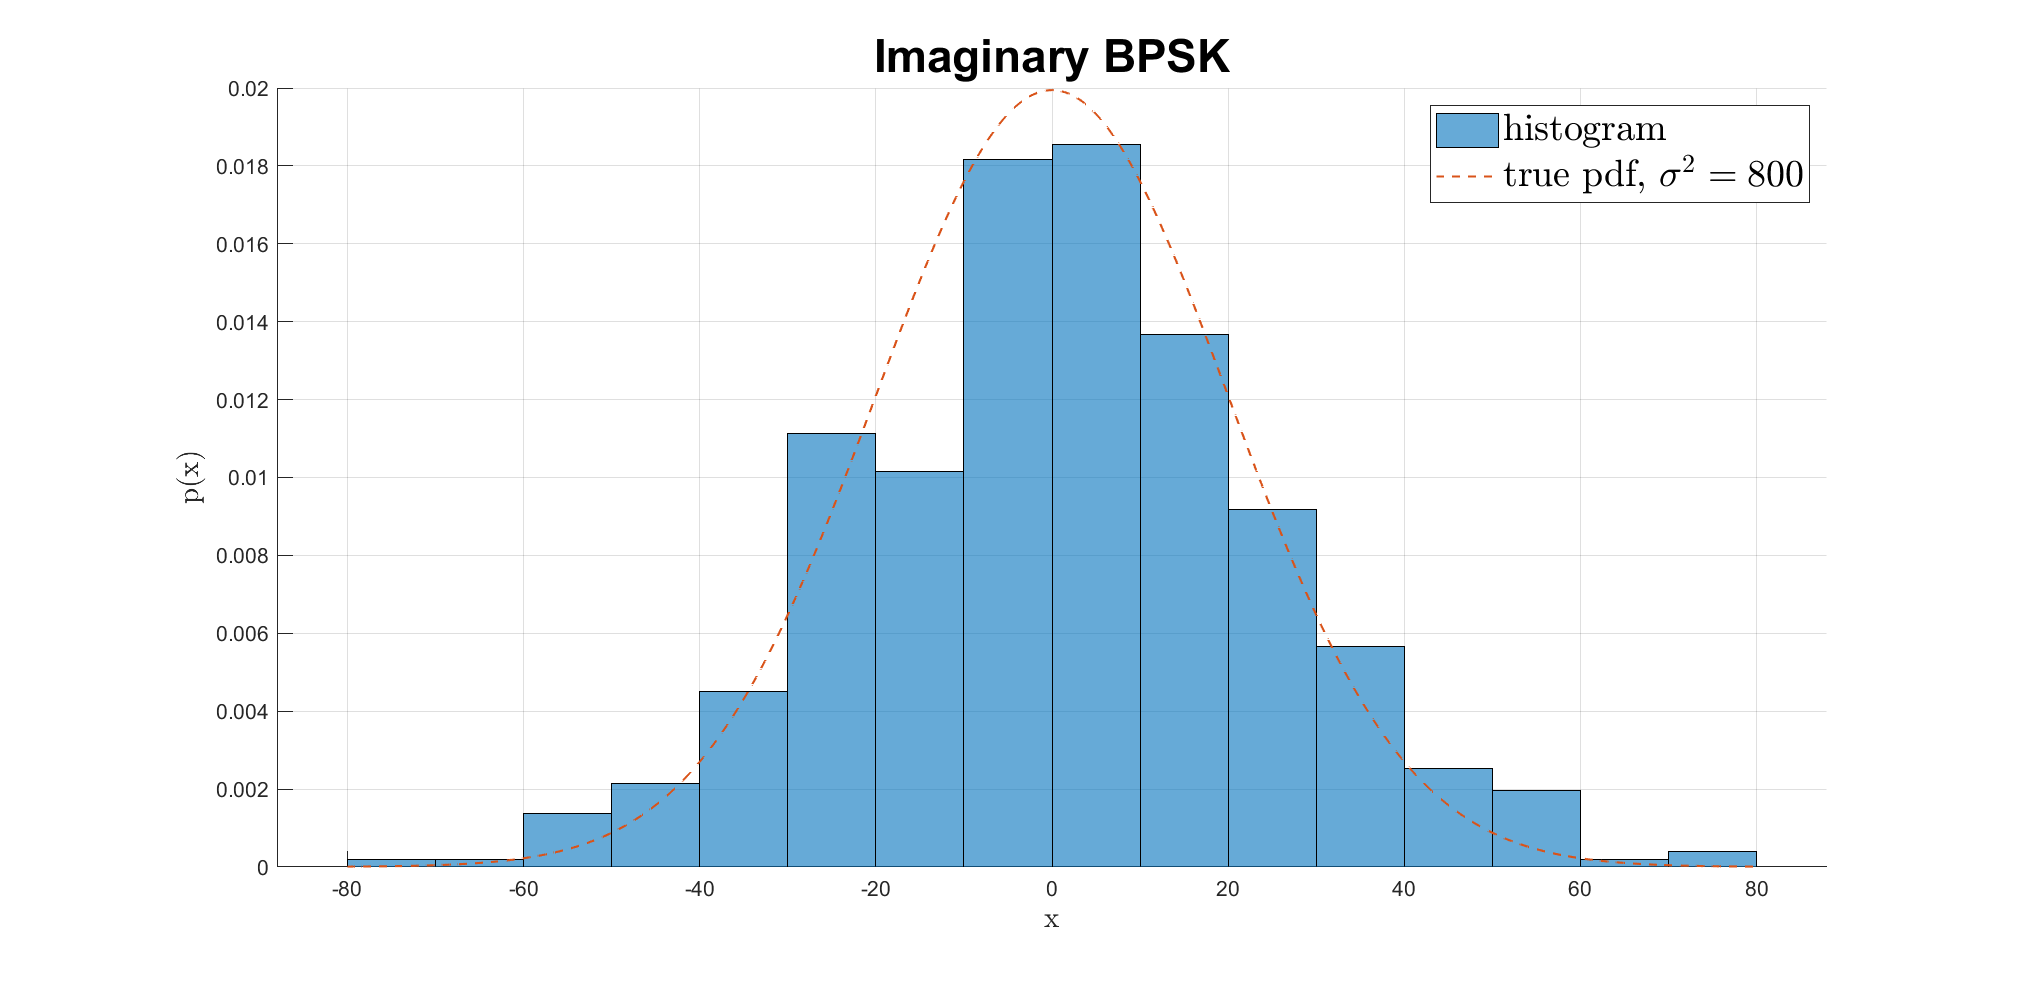
\includegraphics[width=.8\linewidth]{figures/im_bpsk.eps}
        \caption{The histogram of Im(S(k))$~$BPSK}
        \label{fig:im_bpsk}
    \end{subfigure}
    \caption{The histograms compared to pdf of Gaussian}
    \label{fig:gauss}
\end{figure}
In the calculations of the variance and expected value for the four distributions the results were:
\begin{table}[ht]
\centering
\begin{tabular}{|l|l|l|l|}
\hline
\multicolumn{2}{|l|}{Gaussian} & \multicolumn{2}{|l|}{BPSK}\\ \hline
$\mathbb{E}\{s[n]$\} & $\mathbb{E}\{s_{r}[n]s_{i}[n]$\} & $\mathbb{E}\{s[n]$\} & $\mathbb{E}\{s_{r}[n]s_{i}[n]$\}\\
\hline
$0.53767-j2.0817\cdot10^{-16}$ & $1.707\cdot10^{-15}$ & $1-j6.5919\cdot10^{-17}$ & $2.4425\cdot10^{-15}$\\ 
\hline
\end{tabular}
\caption{Shows the expected value for each distributions}
\end{table}
\newline However looking at the histogram it seems like the expected value is approximately at $0$ anyways for all the four distributions.

\subsection{Task 2: One-sample-detector}
In this task only one sample is used meaning that the detection problem is in this case:
\begin{align}
    H_0 &: x[0] = w[0]\nonumber\\
    H_1 &: x[0] = s[0]+w[0]\nonumber
\end{align}
It is given from the problem that $w\thicksim\mathbb{C}\mathcal{N}(0, \sigma_w^2)$ and $s\thicksim\mathbb{C}\mathcal{N}(\mu_s, \sigma_s^2)$ which means that under $H_0$, $x$ is from same distribution as $w$ and thus a complex gaussian with same mean and variance as $w$. Under $H_1$, which is a sum of two complex gaussian distribution, $x$ also is from a complex gaussian distribution. However the mean and variance needs to be calculated to adjust for both distributions.
The mean of $x[0]$ under $H_1$ is
\begin{align}
    \mathbb{E}\{x[0]\} & = \mathbb{E}\{s[0]+w[0]\}\nonumber\\
    & = \mathbb{E}\{s[0]\} + \mathbb{E}\{w[0]\}\nonumber\\
    & = \mu_s + 0 = \mu_s\nonumber
\end{align} 
The variance of $x[0]$ under $H_1$ is
\begin{align}
    \mathrm{Var}\{x[0]\} & = \mathrm{Var}\{s[0]+w[0]\}\nonumber\\
    & = \mathrm{Var}\{s[0]\} + \mathrm{Var}\{w[0]\}\nonumber\\
    & = \sigma_s^2+\sigma_w^2\nonumber
\end{align}
Meaning that
\begin{align}
    p(x;H_0) & = p_0(x) = \frac{1}{\sigma_w^2\pi}e^{-\frac{|x|^2}{\sigma_w^2}}\\
    p(x;H_1) & = p_1(x) = \frac{1}{(\sigma_w^2+\sigma_s^2)\pi}e^{-\frac{|x-\mu_s|^2}{\sigma_s^2+\sigma_w^2}}
\end{align}
Setting up the LRT:
\begin{align}
    L(x) & = \frac{p_1(x[0])}{p_0(x[0])} = \frac{\frac{1}{(\sigma_w^2+\sigma_s^2)\pi}e^{-\frac{|x[0]-\mu_s|^2}{\sigma_s^2+\sigma_w^2}}}{\frac{1}{\sigma_w^2\pi}e^{-\frac{|x[0]|^2}{\sigma_w^2}}}\nonumber\\
    & = \frac{\sigma_w^2}{\sigma_w^2+\sigma_s^2}e^{-\frac{1}{\sigma_w^2+\sigma_s^2}|x[0]-\mu_s|^2+\frac{1}{\sigma_w^2}|x[0]|^2}\nonumber
\end{align}
Since it is given that $\mu_s \approx 0$ this can be used to simplify the caluclations. The decision rule is to choose $H_1$ when $L(x[0]) \geq \lambda$, since $L(x[0])$ is a monotonically increasing function then the inequality holds for $\ln L(x[0]) \geq \ln\lambda$.
\begin{align}
    \ln L(x[0]) = \ln (\sigma_w^2)-\ln (\sigma_w^2+\sigma_s^2) & -\frac{1}{\sigma_w^2+\sigma_s^2}|x[0]|^2 +\frac{1}{\sigma_w^2}|x[0]|^2 \geq \ln\lambda\nonumber\\
    \left(\frac{1}{\sigma_w^2}+\frac{1}{\sigma_s^2+\sigma_w^2}\right)|x[0]|^2 & \geq \ln\lambda-\ln \frac{\sigma_w^2}{\sigma_w^2+\sigma_s^2}\nonumber\\
    |x[0]|^2 = x_R[0]^2+x_I[0]^2 & \geq \frac{\sigma_w^2(\sigma_w^2+\sigma_s^2)}{\sigma_s^2}\left(\ln\lambda-\ln\frac{\sigma_w^2}{\sigma_w^2+\sigma_s^2}\right) = \lambda'\nonumber
\end{align}
This also means that the decision rule is to choose $H_1$ when $|x[0]|^2\geq\lambda'$ and choose $H_0$ when $|x[0]|^2<\lambda'$ where
\begin{equation}
    \lambda' = \frac{\sigma_w^2(\sigma_w^2+\sigma_s^2)}{\sigma_s^2}\left(\ln\lambda-\ln \frac{\sigma_w^2}{\sigma_w^2+\sigma_s^2}\right)
\end{equation}\label{eq:lambda_prime}

\subsection{Task 3: Performance of the one-sample detector}
\begin{figure}[ht]
    \begin{subfigure}{.5\textwidth}
        \centering
        % include first image
        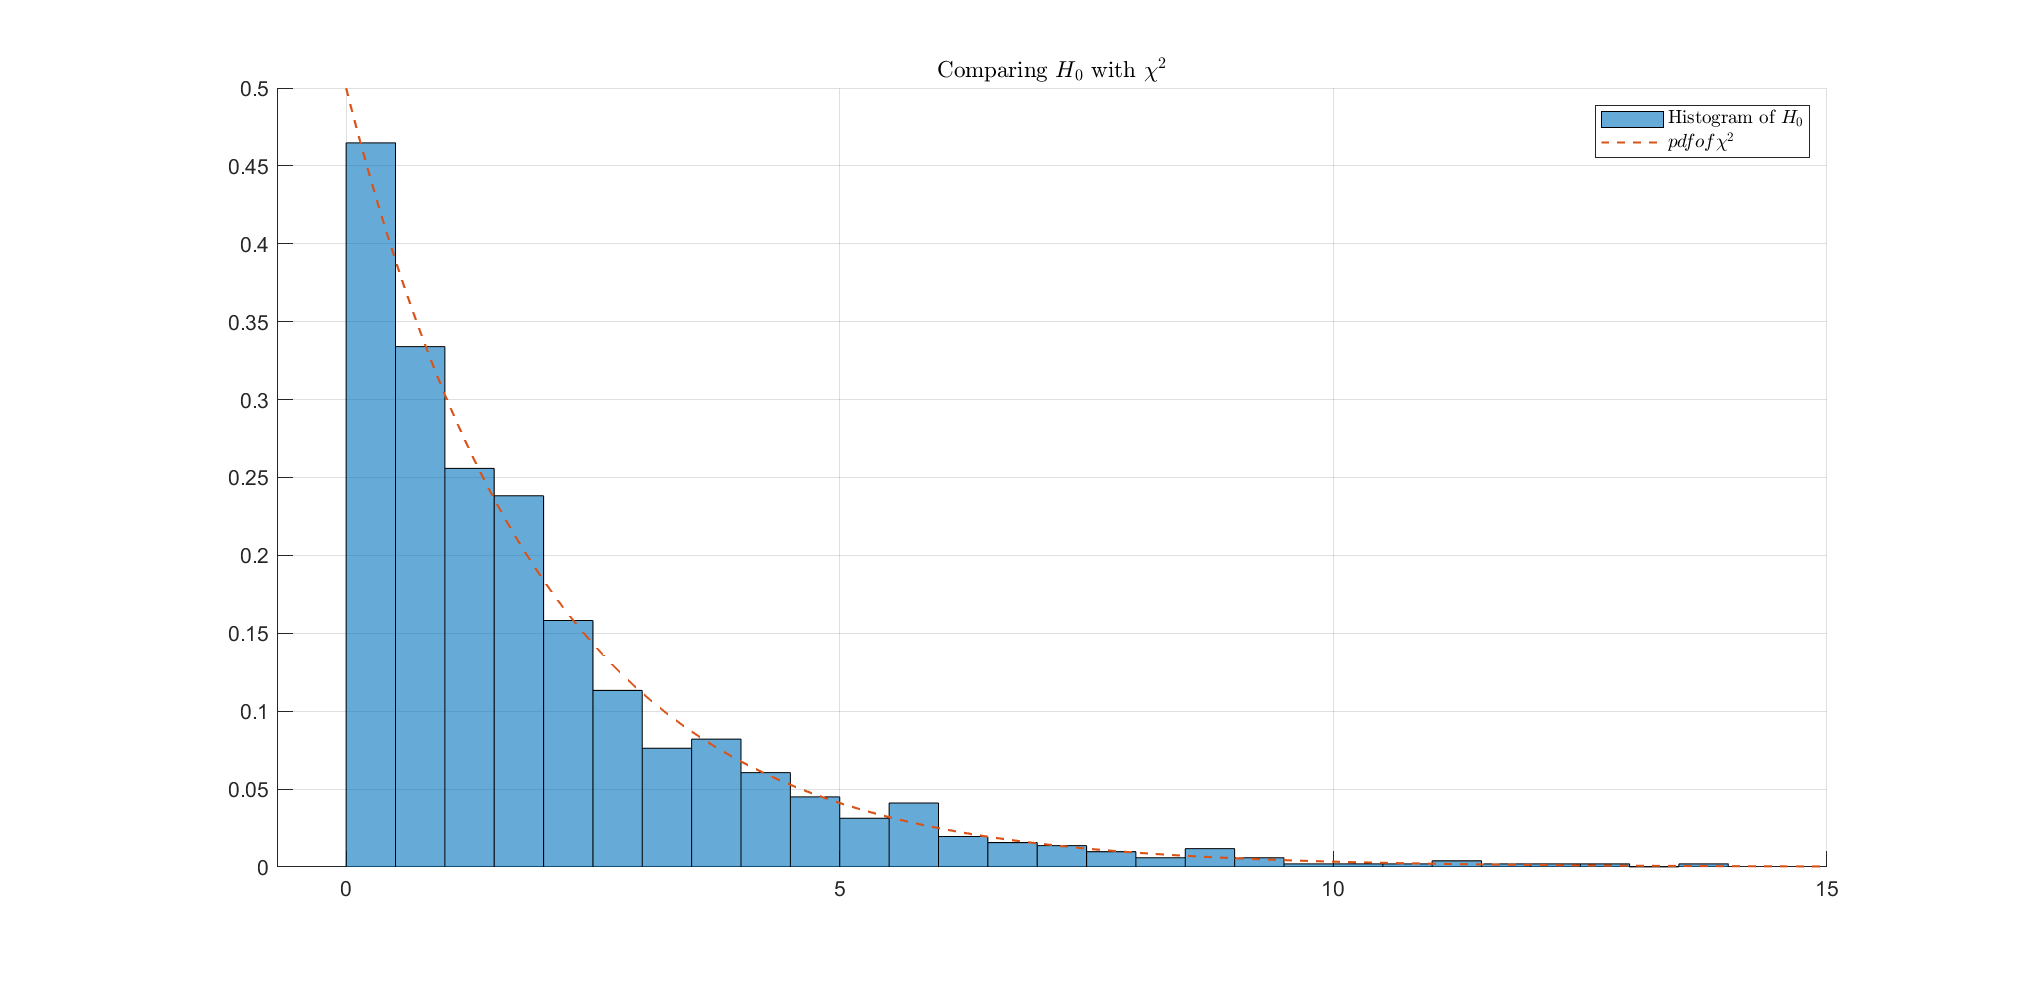
\includegraphics[width=.8\linewidth]{figures/chi_square_h0.eps}  
        \caption{The histogram of \eqref{eq:chi_sq_h0}}
        \label{fig:chi_sq_h0}
    \end{subfigure}
    \begin{subfigure}{.5\textwidth}
        \centering
        % include second image
        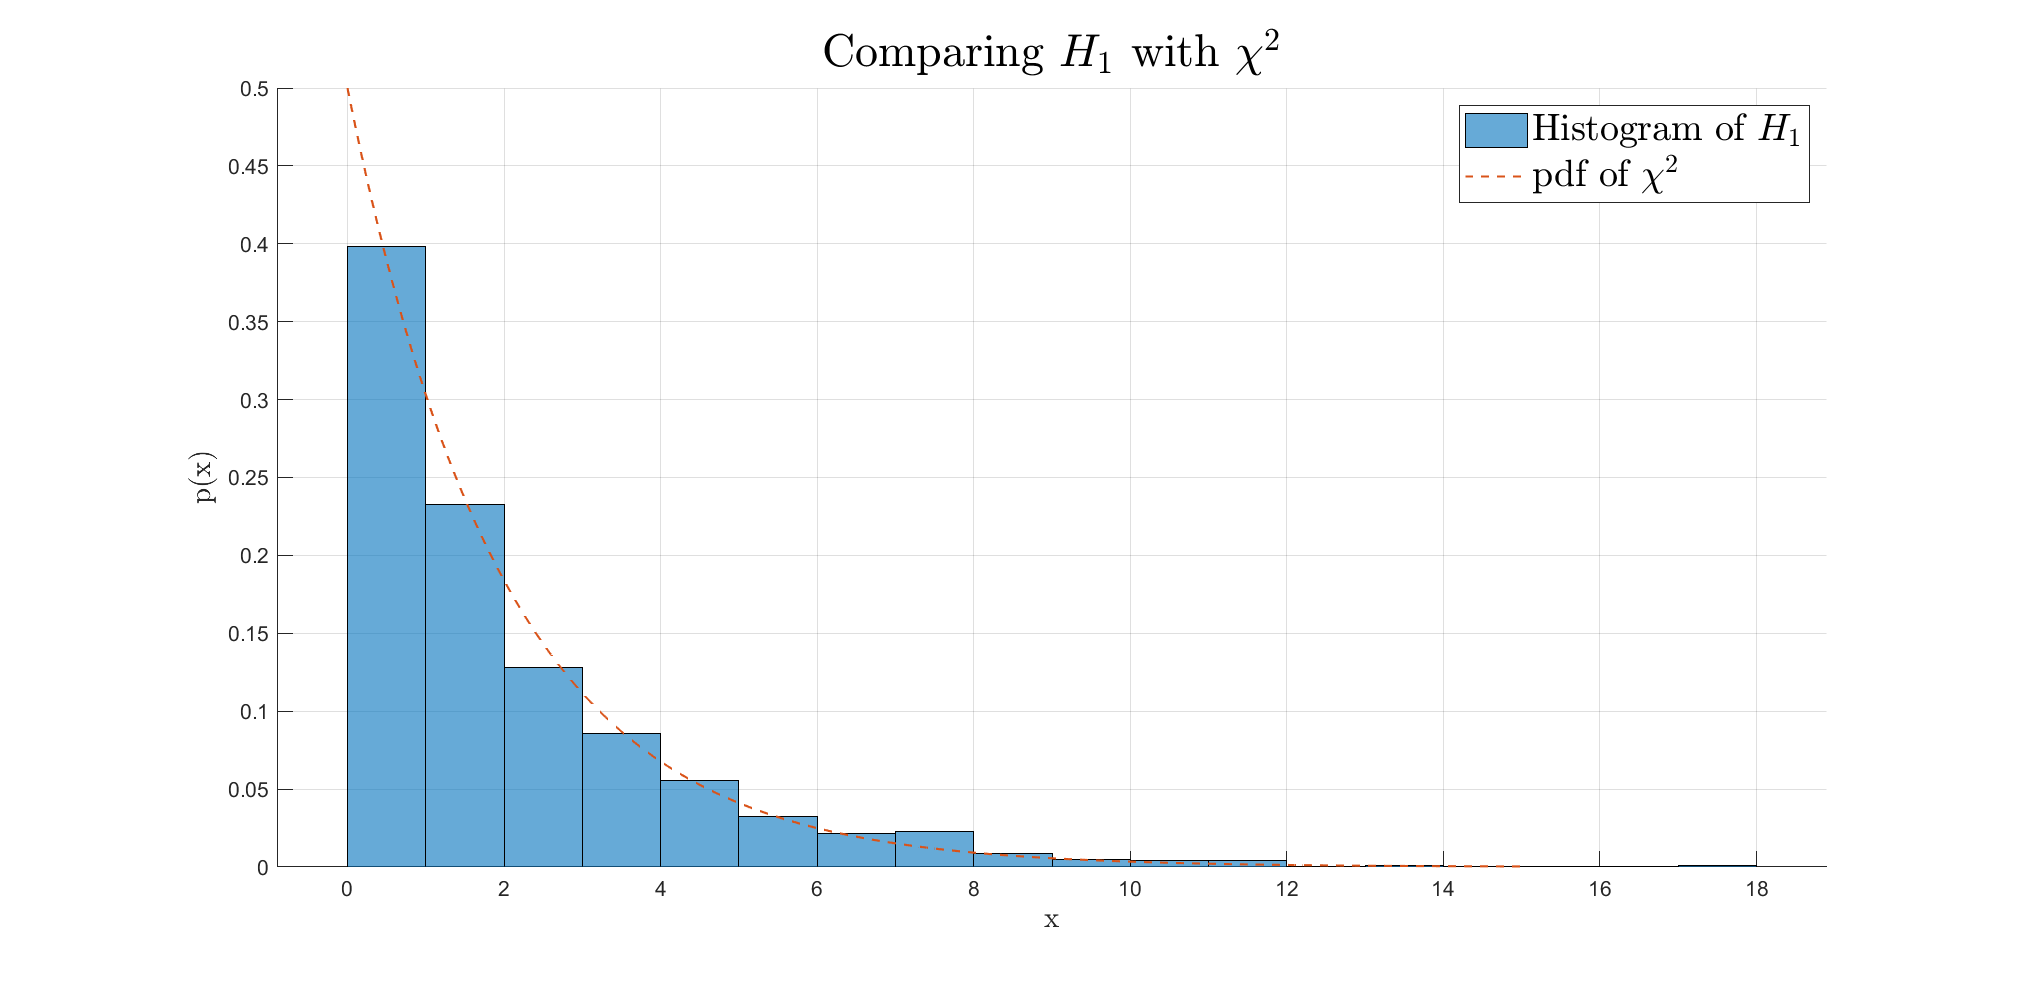
\includegraphics[width=.8\linewidth]{figures/chi_square_h1.eps}  
        \caption{The histogram of \eqref{eq:chi_sq_h1}}
        \label{fig:chi_sq_h1}
    \end{subfigure}
\end{figure}
The histogram in \ref{fig:chi_sq_h0} and \ref{fig:chi_sq_h1} shows that $|x[0]|^2$ is $\chi^2$-distributed with 2 degrees of freedom both under $H_0$ and $H_1$ and the difference between $H_0$ and $H_1$ is essentially the constant scaling factor given by the variances $\sigma_w^2$ and $\sigma_s^2$.
Calculating the probability for the false alarm gives
\begin{align}
    P_{FA} & = \text{Prob}\{|x[0]|\geq\lambda'\big\vert H_0\}\nonumber\\
    & = \int_{\lambda'}^{\infty}\frac{e^{-\frac{2x[0]}{2\sigma_w^2}}}{\sigma_w^2}dx[0]\nonumber\\
    & = -\frac{\sigma_w^2}{\sigma_w^2}e^{-\frac{x[0]}{\sigma_w^2}}\bigg\rvert_{\lambda'}^{\infty}\nonumber\\
    & = e^{-\frac{\lambda'}{\sigma_w^2}}\nonumber
\end{align}
Which only holds when $\lambda'>0$.\\
Furthermore the probability for detection is
\begin{align}
    P_D & = \text{Prob}\{|x[0]|\geq\lambda'\big\vert H_1\}\nonumber\\
    & = \int_{\lambda'}^{\infty}\frac{e^{-\frac{x[0]}{\sigma_w^2+\sigma_s^2}}}{\sigma_w^2+\sigma_s^2}dx[0]\nonumber\\
    & = -\frac{\sigma_w^2+\sigma_s^2}{\sigma_w^2+\sigma_s^2}e^{-\frac{x[0]}{\sigma_w^2+\sigma_s^2}}\bigg\rvert_{\lambda'}^{\infty}\nonumber\\
    & = e^{-\frac{\lambda'}{\sigma_w^2+\sigma_s^2}}\nonumber
\end{align}
Which also only holds for $\lambda'>0$\\

\subsection{Task 4: Generalized for multiple samples}
We take the one-sample-detector a step further and generalize it to use it for multiple samples. That is that the likelihood function is used to calculate the LRT so that we get
\begin{align}
    \ln L(x) & = \ln\prod_{n=0}^{K-1}\frac{1}{(\sigma_w^2+\sigma_s^2)\pi}e^{-\frac{|x(n)|^2}{\sigma_s^2+\sigma_w^2}}-\ln\prod_{n=0}^{K-1}\frac{1}{\sigma_w^2\pi}e^{-\frac{|x(n)|^2}{\sigma_w^2}}\nonumber\\
    & = \sum_{n=0}^{K-1}\left(\ln\frac{\sigma_w^2}{\sigma_w^2+\sigma_s^2} + \frac{|x(n)|^2}{\sigma_w^2}-\frac{|x(n)|^2}{\sigma_w^2+\sigma_s^2} \right)\nonumber\\
    & = \sum_{n=0}^{K-1}\left(\ln\frac{\sigma_w^2}{\sigma_w^2+\sigma_s^2} + \frac{\sigma_s^2}{\sigma_w^2(\sigma_w^2+\sigma_s^2)}|x(n)|^2\right)\geq\ln\lambda\nonumber
\end{align}
So the decision rule ends up being to choose $H_1$ when
\begin{equation}
    T(\mathbf{x}) = \sum_{n=0}^{K-1}|x(n)|^2 \geq \frac{\sigma_w^2(\sigma_w^2+\sigma_s^2)}{\sigma_s^2}\left(\ln\lambda-K\ln\frac{\sigma_w^2}{\sigma_w^2+\sigma_s^2}\right) = \lambda'
\end{equation}
Here $T(\mathbf{x})$ is a sum of $K$ complex Gaussian squared, meaning the pdf in this case is a $\chi^2$-distribution with $2K$ degrees of freedom. This means that
\begin{align}
    P_D & = \int_{\lambda'}^{\infty}\frac{x^{K-1}e^{-\frac{x}{\sigma_w^2+\sigma_s^2}}}{(\sigma_w^2+\sigma_s^2)^K\Gamma(K)}dx\nonumber\\
    & = \frac{1}{(\sigma_w^2+\sigma_s^2)^K\Gamma(K)}\int_{\lambda'}^{\infty}x^{K-1}e^{-\frac{x}{\sigma_w^2+\sigma_s^2}}dx\nonumber\\
    & = Q\left(\frac{\lambda'}{\sigma_w^2+\sigma_s^2}\right)
\end{align}
Differentiating the integral with respect to $\lambda'$ it shows that $P_D$ is strictly decreasing and has extremal points at $\lambda'=0\vee\lambda'=\infty$. Which essentially means that $P_D$ is maximized when $\lambda'\in[0,\infty)$ is as close to $0$ as possible. For the false alarm with the upper limit $\alpha_0$, its cumulative distribution function is
\begin{align}
    P_{FA} & = \frac{1}{(\sigma_w^2)^K\Gamma(K)}\int_{\lambda'}^{\infty}x^{K-1}e^{-\frac{x}{\sigma_w^2}}dx\nonumber\\
    & = Q\left(\frac{\lambda'}{\sigma_w^2}\right) \leq \alpha_0
\end{align}

Which means that for the inequality to hold in addition to maximize the power of the test, need to choose $\lambda' >= \sigma_w^2Q^{-1}\left(\alpha_0\right)$. Essentially choosing $\lambda' = \sigma_w^2Q^{-1}\left(\alpha_0\right)$ to minimize $P_D$. Inserting this to get the expression for $P_D$.
\begin{equation}
    P_D = Q(\frac{\sigma_w^2}{\sigma_w^2+\sigma_s^2}Q^{-1}\left(\alpha_0\right))
\end{equation}

\subsection{Task 5: Performance of the general detector}
$\chi^2(k)$ is a special case of the Gamma distribution where it has $k/2$ degrees of freedom. Using this and the fact that $Q\sim\chi^2$ has the property that $cQ\sim Gamma(k/2, 2c)$. $T(\mathbf{x})$ has $K$ degrees of freedom in the Gamma distribution. Furthermore under $H_0$, $T(\mathbf{x})$ is scaled such that $c = \frac{\sigma_w^2}{2}$ which gives the point distribution function
\begin{equation}
    p(x) = \frac{x^{K-1}e^{-\frac{x}{\sigma_w^2}}}{\Gamma(K)\sigma_w^{2K}}
\end{equation}
Similarly for $T(\mathbf{x})$ under $H_1$ has the scaling constant $c = \frac{\sigma_w^2+\sigma_s^2}{2}$ and thus the point distribution function
\begin{equation}
    p(x) = \frac{x^{K-1}e^{-\frac{x}{\sigma_w^2+\sigma_s^2}}}{\Gamma(K)(\sigma_w^{2}+\sigma_s^2)^K}
\end{equation}.\\
In figure \ref{fig:roc} the curves become better for increasing doF. This means that if the test statistic $T(\mathbf{x})$ has more samples, the power of the test gets better.
\begin{figure}
    \centering
    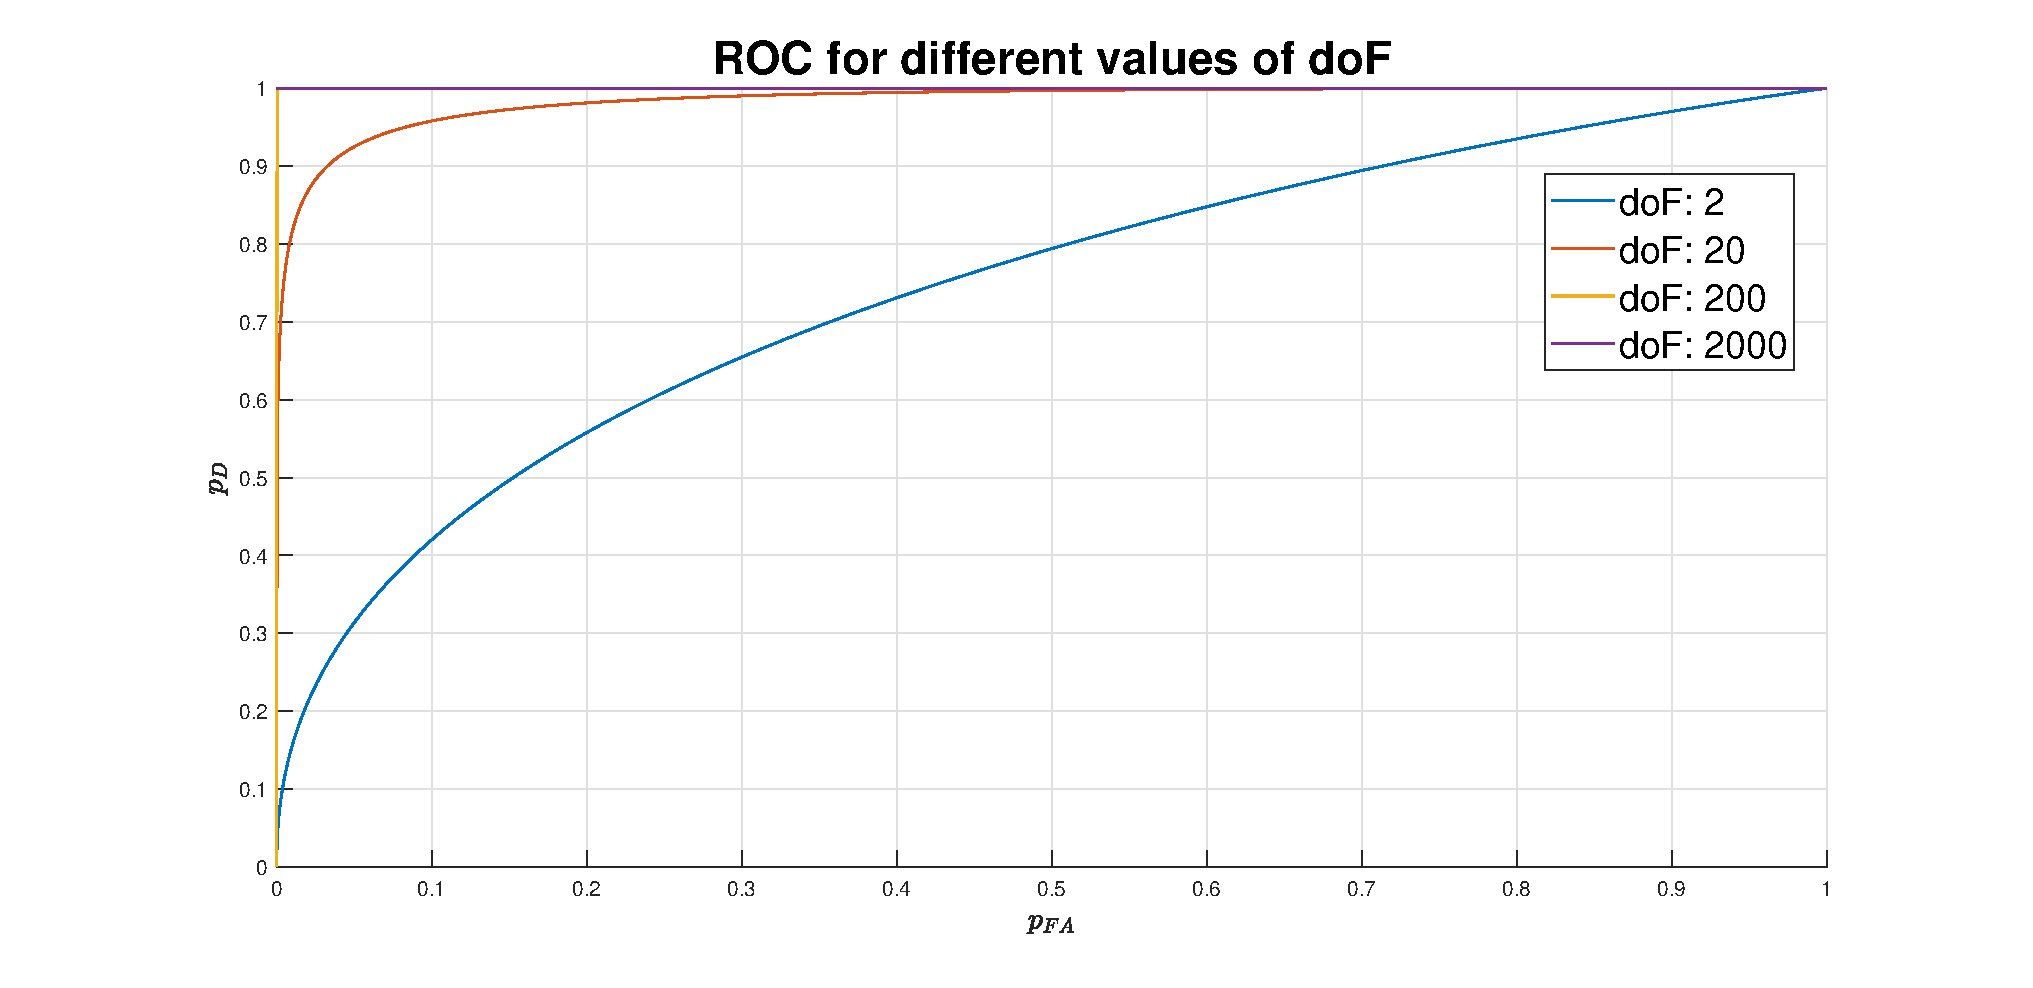
\includegraphics[width=\textwidth]{figures/roc2.eps}
    \caption{The receiver operating characteristics with different doF}
    \label{fig:roc}
\end{figure}

\subsection{Task 6: Central limit theorem}
By the central limit theorem that states that for $T(\mathbf{x}) = \sum_{n=0}^{K-1}|x[n]|^2$, that $T(\mathbf{x})$ converges to a Gaussian distribution when $|x[n]|^2$ comes from a independent identical distribution with finite expected value $\mu$ and finite variance $\sigma^2$. Already know that $|x[n]|$ is complex gaussian and iid for each sample $n = 0, \dots, K-1$, so $|x[n]|^2$ is also iid.\\
\begin{figure}
    \centering
    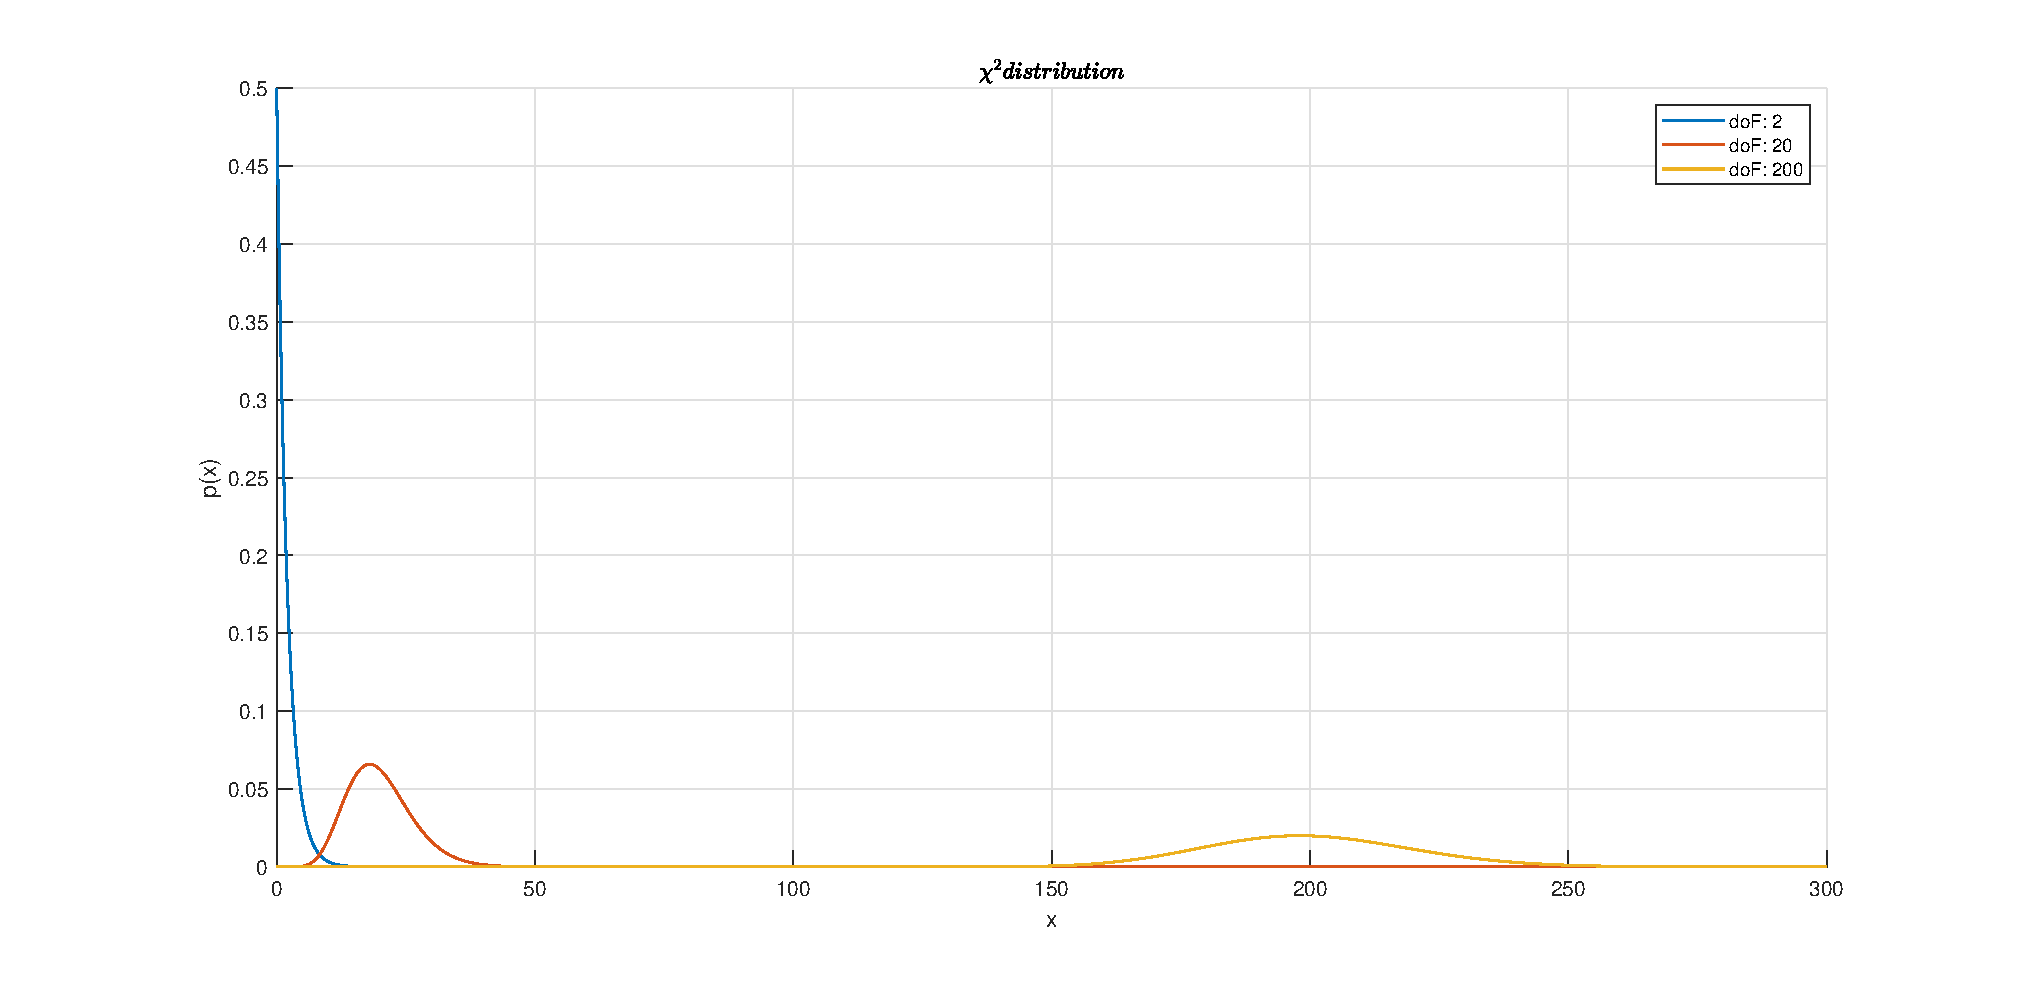
\includegraphics[width=\textwidth]{figures/chi_square.eps}
    \caption{The pdf of $\chi^2$ for different degrees of freedom}
    \label{fig:chitogauss}
\end{figure}
In figure \ref{fig:chitogauss} notice that for higher degrees of freedom, which essentially means for more samples, the pdf of the $\chi^2$ distributions looks more and more like the Gaussian distribution with mean equal to the degrees of freedom.\\
In this case the mean is
\begin{align}
    \hat{\mu} = \mathbb{E}\left\{T(\mathbf{x})\right\} & = \mathbb{E}\{\sum_{n=0}^{K-1}|x[n]|^2\}\nonumber\\
    & = \sum_{n=0}^{K-1}\mathbb{E}\{|x[n]^2|\}\nonumber\\
    & = \sum_{n=0}^{K-1}(\text{Var}\{|x[n]|\}+\mathbb{E}\{|x[n]|\}^2)\nonumber\\
    & = \begin{cases}
    K\sigma_w^2, & \text{under} H_0\\
    K(\sigma_w^2+\sigma_s^2), & \text{under} H_1
    \end{cases}
\end{align}
and the variance is
\begin{align}
    \hat{\sigma^2} = \mathrm{Var}\left\{T(\mathbf{x})\right\} & = \mathrm{Var}\{\sum_{n=0}^{K-1}|x[n]|^2\}\nonumber\\
    & = \sum_{n=0}^{K-1}\mathrm{Var}\{|x[n]|^2\}\nonumber\\
    & = \sum_{n=0}^{K-1}(\mathbb{E}\{|x[n]|^4\}-\mathbb{E}\{|x[n]|^2\}^2\nonumber)\\
    & = \begin{cases}
    K\sigma_w^4, & \text{under} H_0\\
    K(\sigma_s^2+\sigma_w^2)^2, & \text{under} H_1
    \end{cases}
\end{align}


Which gives the pdf of a normal Gaussian for each of the cases as
\begin{equation}
    f(x) = \frac{1}{\sqrt{2\pi\hat{\sigma}^2}}e^{-\frac{1}{2}\left(\frac{x-\hat{\mu}}{\hat{\sigma}}\right)^2}
\end{equation}
This results in the two figures in for $T(\mathbf{x})$ under $H_0$ and $H_1$ in figure \ref{fig:clt}
\begin{figure}[ht]
    \begin{subfigure}{\textwidth}
        \centering
        % include first image
        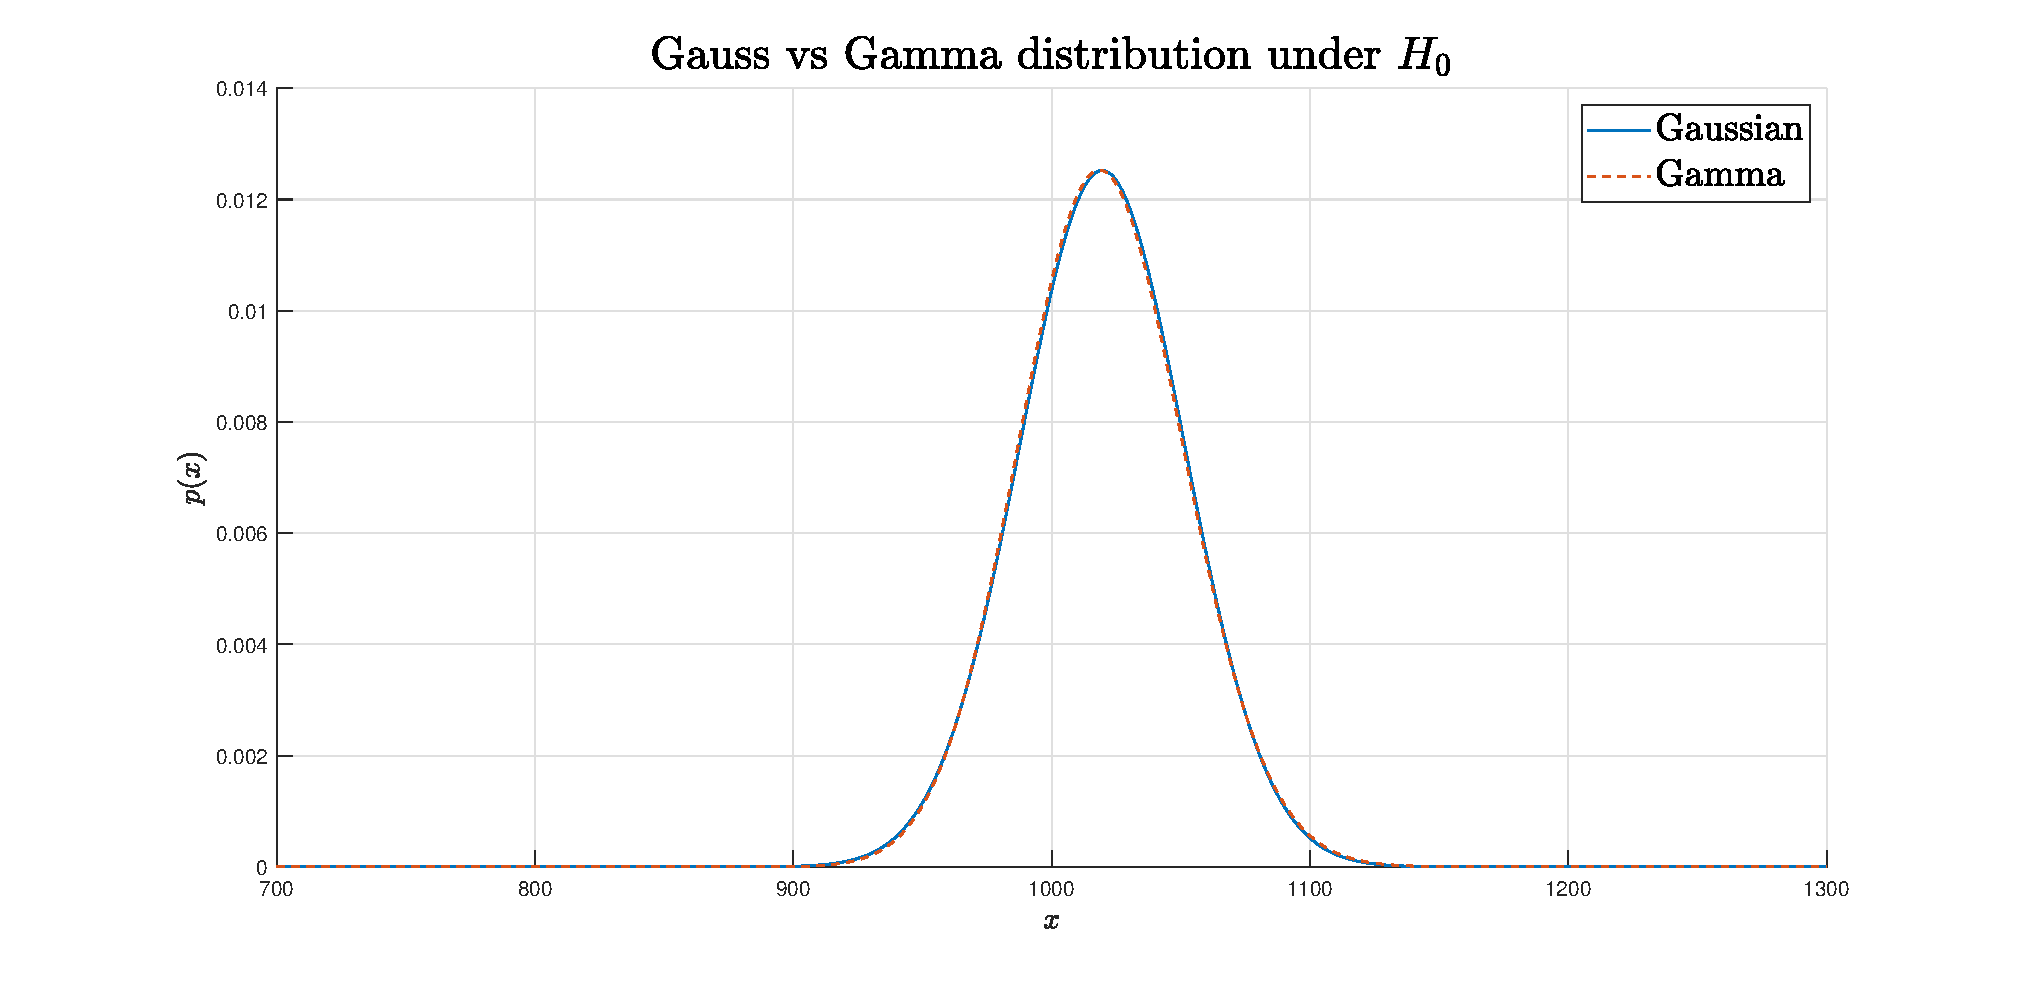
\includegraphics[width=.8\linewidth]{figures/gauss_vs_gamma_h0.eps}  
        \caption{Normal vs Gamma distribution under $H_0$}
        \label{fig:gaussvsgamma_h0}
    \end{subfigure}
    \begin{subfigure}{\textwidth}
        \centering
        % include second image
        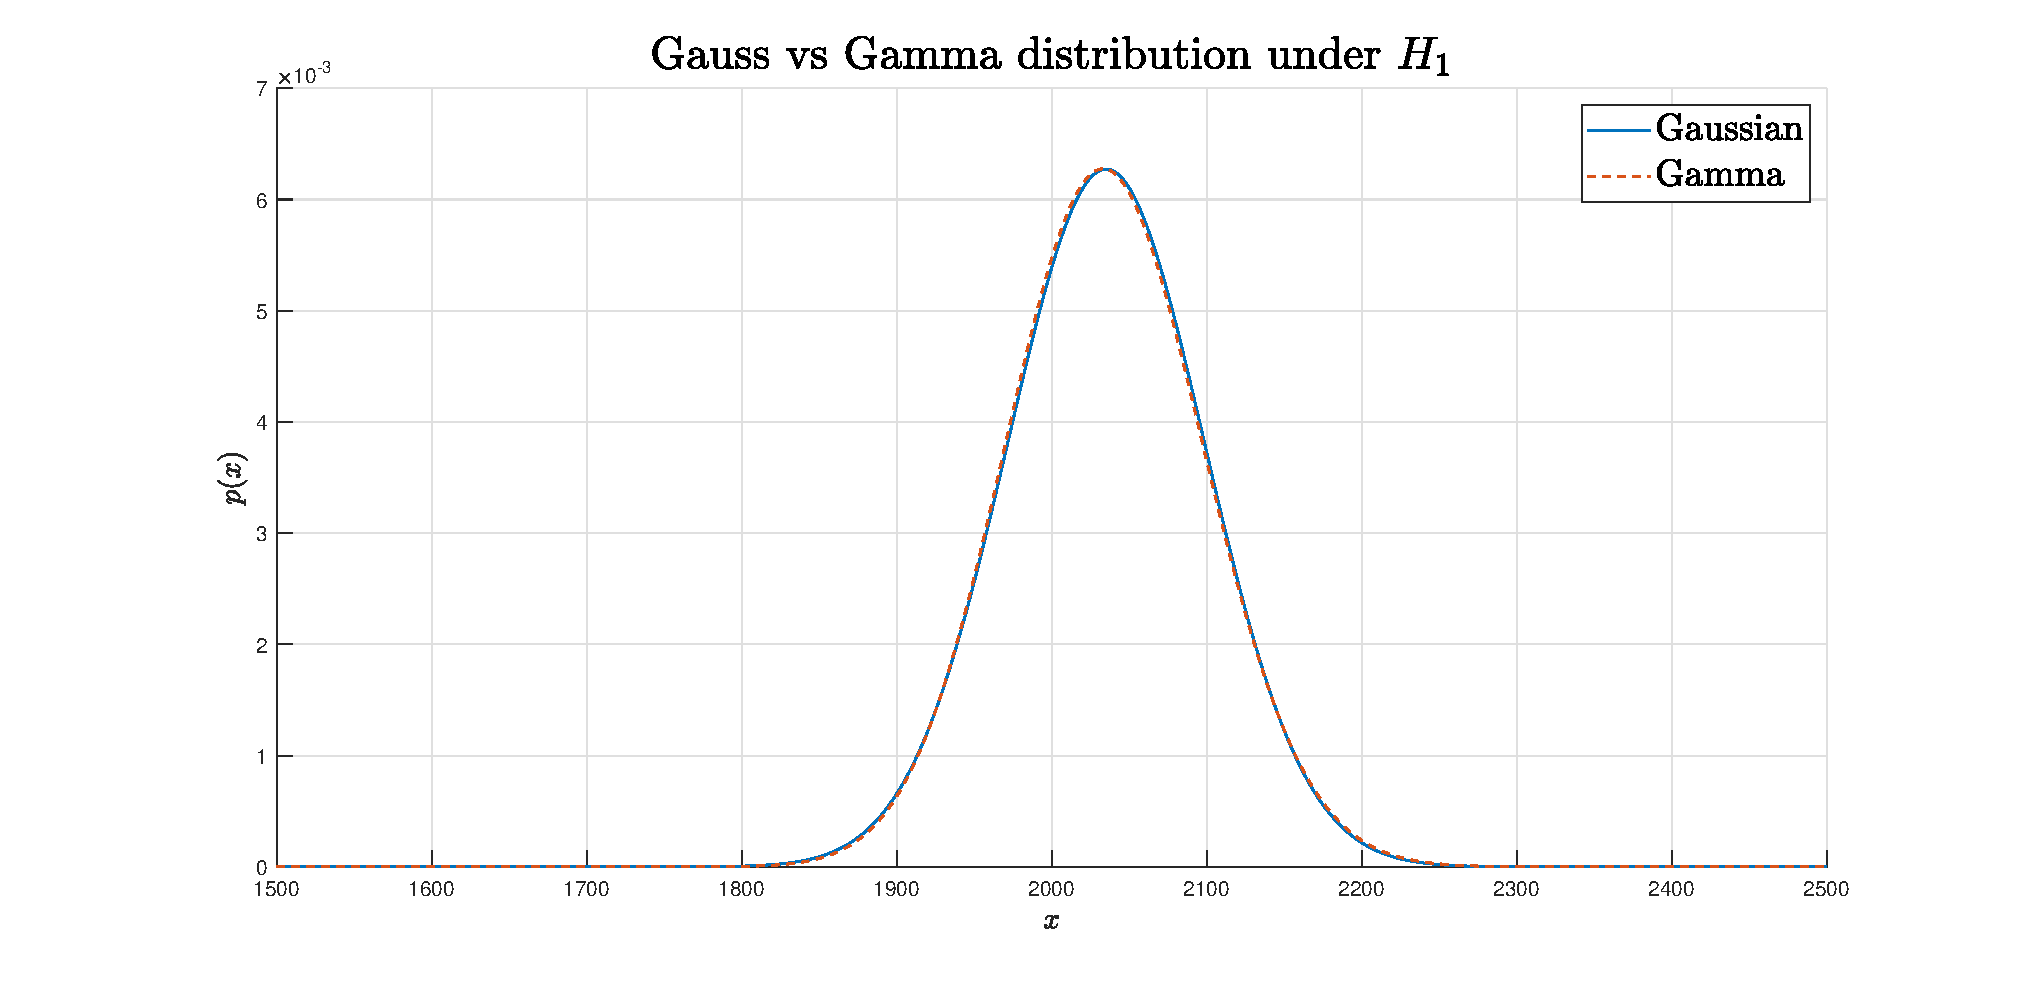
\includegraphics[width=.8\linewidth]{figures/gauss_vs_gamma_h1.eps}  
        \caption{Normal vs Gamma distribution under $H_1$}
        \label{fig:gaussvsgamma_h1}
    \end{subfigure}
    \caption{}
    \label{fig:clt}
\end{figure}
Resulting in more general distribution that can be used for detectors on the same form as $T(\mathbf{x})$, when it is a sum of iid random variables. Using this as the pdf when calculating the $P_{FA}$ and $P_D$ results in \ref{fig:pfavspdaslambda}
\begin{figure}
    \centering
    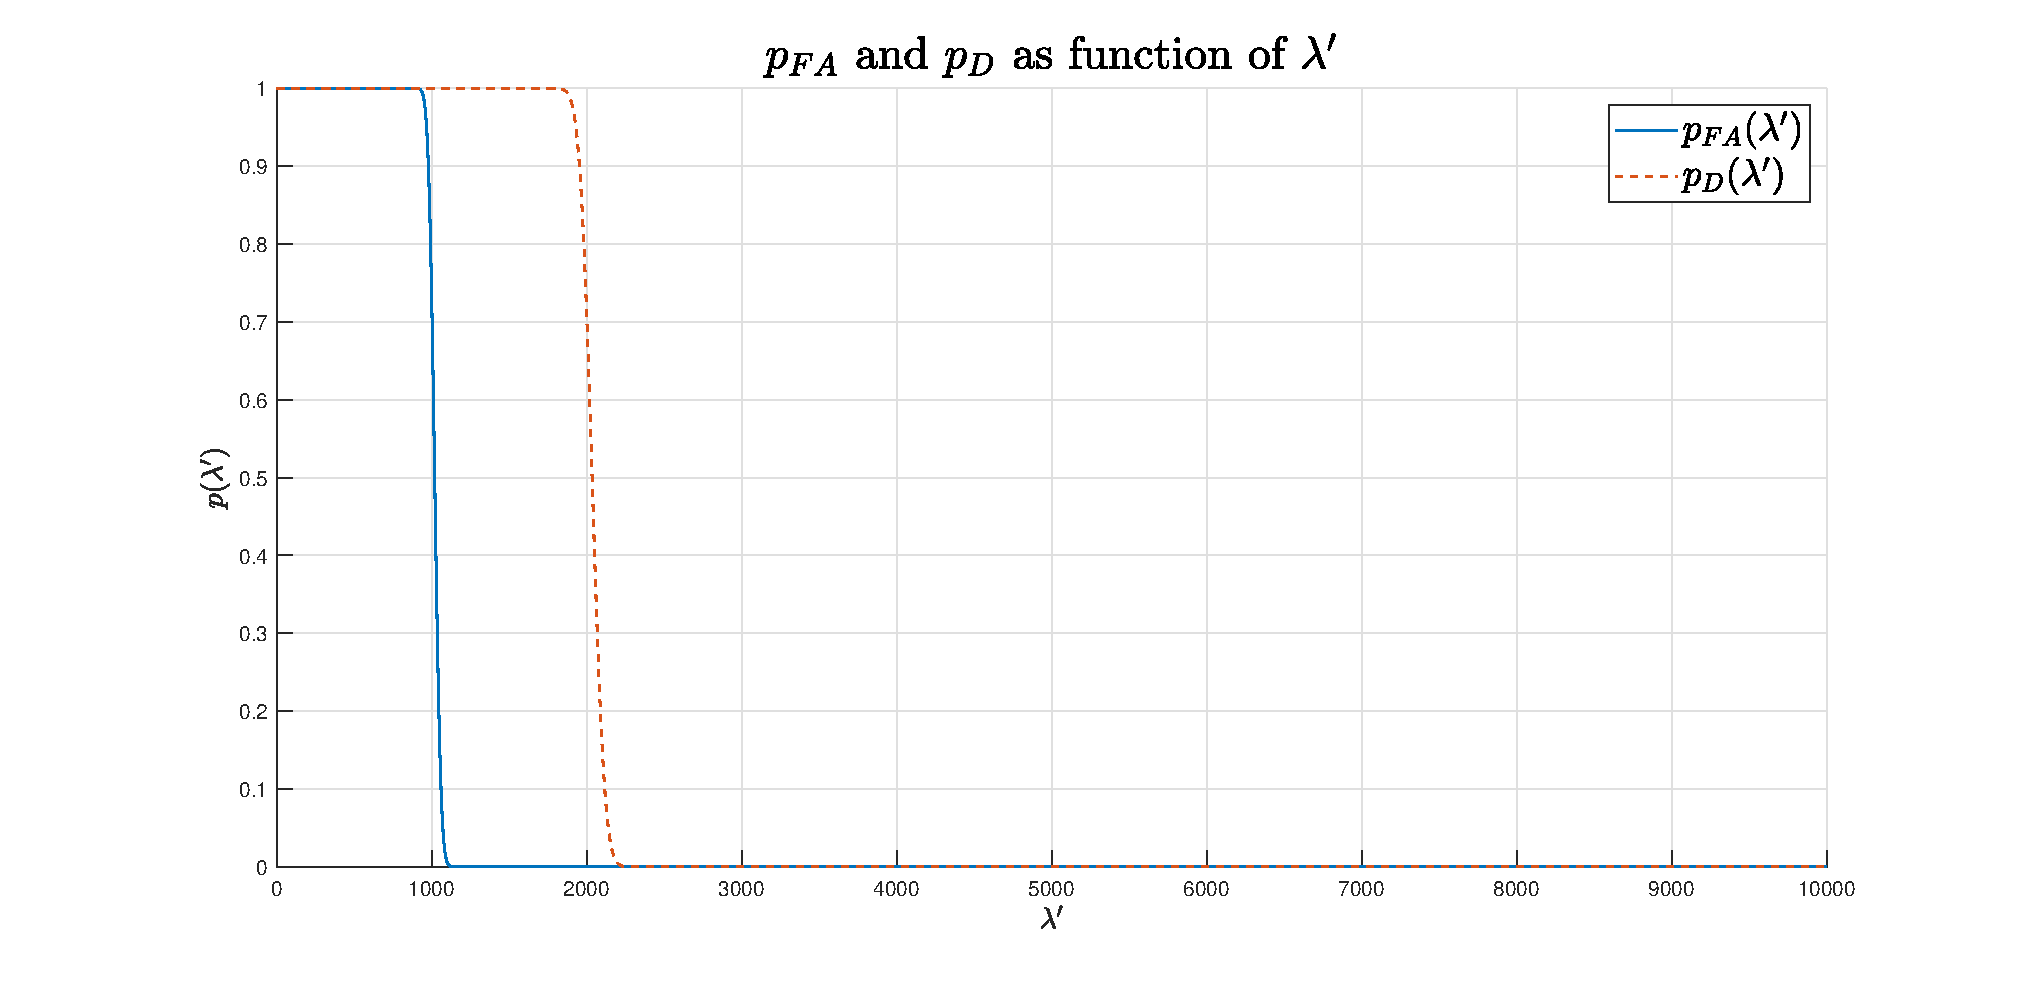
\includegraphics[width=\textwidth]{figures/gauss_lambda_pfa_pd.eps}
    \caption{Showing how $P_{FA}$ and $P_D$ change with $\lambda'$}
    \label{fig:pfavspdaslambda}
\end{figure}

One can see that the results are quite similar to the exact $P_{D}$ and $P_{FA}$

\begin{figure}
    \centering
    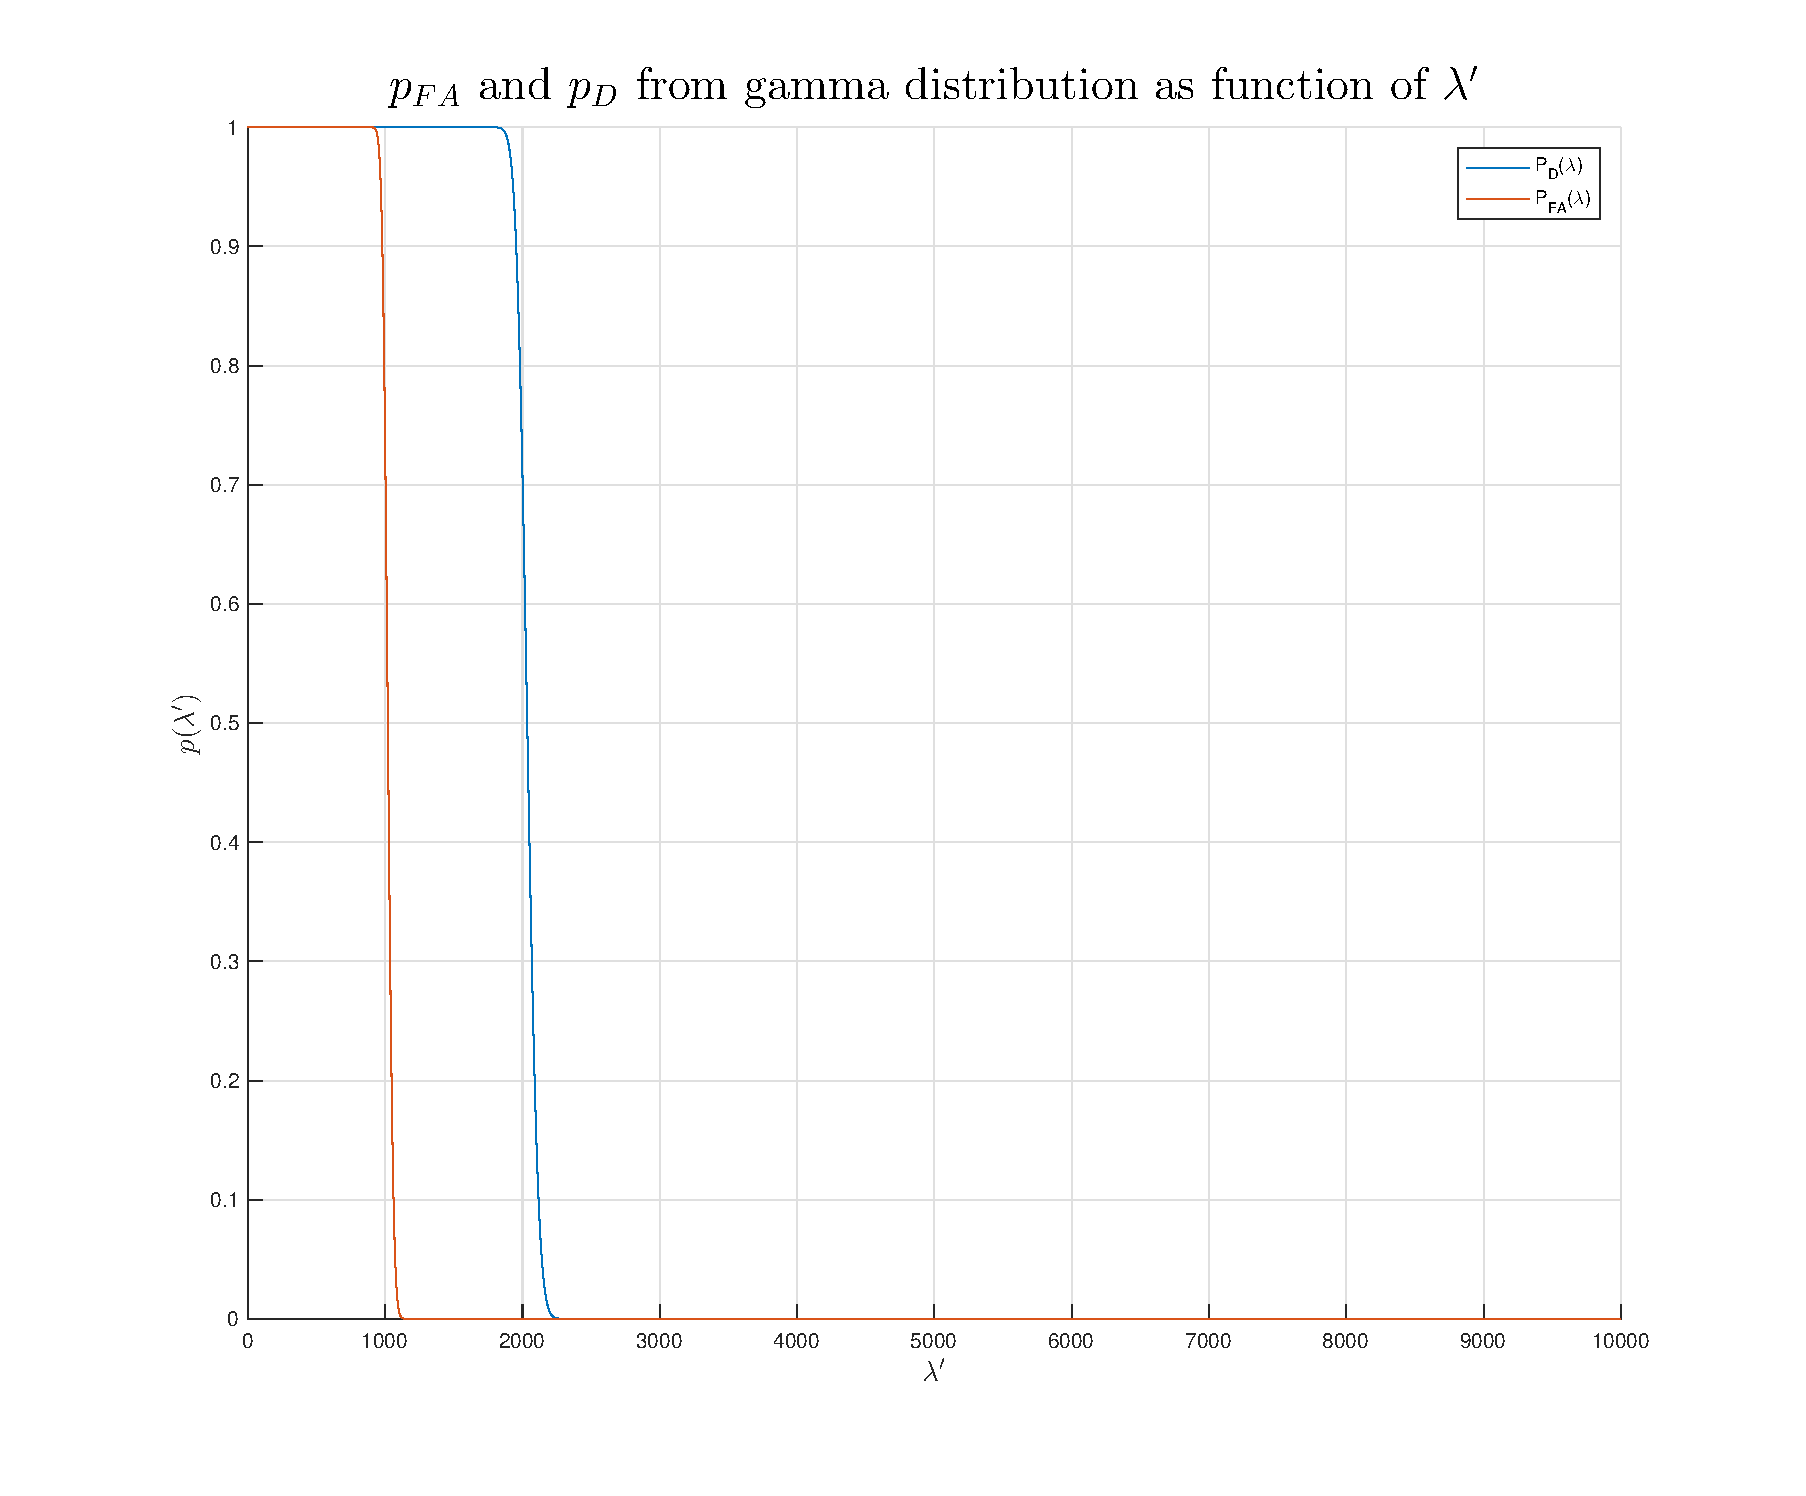
\includegraphics[width=\textwidth]{figures/p-d-fa-gauss.eps}
    \caption{Showing how the exact $P_{FA}$ and $P_D$ change with $\lambda'$}
    \label{fig:exactpdpfa}
\end{figure}

\newpage

\subsection{Task 7: Detector complexity}
Using the pdf for Gaussian distribution, to find an expression for $K$.
\begin{align}
    P_{FA} & = 
    \int_{\lambda'}^{\infty}\frac{1}{\sqrt{2\pi K\sigma_w^4}}e^{-\frac{1}{2}\frac{\left(x-K\sigma_w^2\right)^2}{K\sigma_w^4}}\nonumber\\
    & = Q\left(\frac{\lambda'-K\sigma_w^2}{\sqrt{K}\sigma_w^2}\right)
    = \alpha\label{eq:pfagauss}
\end{align}
Solve \eqref{eq:pfagauss} for $\lambda'$ to retrieve
\begin{align}
    \lambda' & = \left(Q^{-1}(\alpha)\sqrt{K}+K\right)\sigma_w^2\label{eq:gausslambdaprime}
    \end{align}
Do the same for $P_D$
\begin{align}
    P_{D} & = 
    \int_{\lambda'}^{\infty}\frac{1}{\sqrt{2\pi K(\sigma_w^2+\sigma_s^2)^2}}e^{-\frac{1}{2}\frac{(x-K(\sigma_w^2+\sigma_s^2))^2}{K(\sigma_w^2+\sigma_s^2)^2}}\nonumber\\
    & = Q\left(\frac{\lambda'-K(\sigma_w^2+\sigma_s^2)}{\sqrt{K(\sigma_w^2+\sigma_s^2)^2}}\right)
    = \beta\label{eq:pdgauss}
\end{align}
Solve \eqref{eq:pdgauss} for $K$, and utilize the result from \eqref{eq:gausslambdaprime} as substitute for $\lambda'$
\begin{align}
    Q^{-1}(\beta) & = \frac{\lambda'-K(\sigma_w^2+\sigma_s^2)}{\sqrt{K(\sigma_w^2+\sigma_s^2)^2}}\nonumber\\
    & = \frac{(Q^{-1}(\alpha)\sqrt{K}+K)\sigma_w^2-K(\sigma_w^2+\sigma_s^2)}{\sqrt{K}(\sigma_w^2+\sigma_s^2)}\nonumber\\
    & = \frac{Q^{-1}(\alpha)\sqrt{K}\sigma_w^2-K\sigma_s^2}{\sqrt{K}(\sigma_w^2+\sigma_s^2)}\nonumber\\
    & = \frac{Q^{-1}(\alpha)\sqrt{K}\sigma_w^2}{\sqrt{K}(\sigma_w^2+\sigma_s^2)}-\frac{K\sigma_s^2}{\sqrt{K}(\sigma_w^2+\sigma_s^2)}\nonumber\\
    \frac{K}{\sqrt{K}}\sigma_s^2 & = Q^{-1}(\alpha)\sigma_w^2-Q^{-1}(\beta)(\sigma_w^2+\sigma_s^2)\nonumber\\
    K & = \left( \frac{Q^{-1}(\alpha)\sigma_w^2-Q^{-1}(\beta)(\sigma_w^2+\sigma_s^2)}{\sigma_s^2}\right)^2
\end{align}
Which gives the amount of samples $K$ needed to attain the limit $P_{FA} = \alpha$ and $P_D = \beta$. Furthermore an observation that can be done is that Q is cumulative function for the standard Gaussian distribution where the mean is $0$ and standard deviation is $1$.






\subsection{Task 8: Test with data}


Using the Gaussian detector for all K samples of the data.

\begin{enumerate}[i]
    \item What is this chapter about
    \item Matlab implementation
    \item Any specific Matlab m-commands used?
    \item A flow-diagram is recommended
    \item Results (use figures/tables if possible)
    \item Discussion of results
    \item Matlab code (documented) in appendix
\end{enumerate}





